\section{Structure validation and comparison}

 At the end of the refinement process of \ttt{metHgb} $\alpha$ subunit (a similar one would be required for $\beta$ subunit), we need to assess the geometry of our $model$ regarding the starting 
volume to detect $model$ controversial elements or $model$ parameters that disagree with the map. Although each refinement program has their own tools to assess the progress of refinement ($Coot$ \ttt{Validate} menu; $Phenix$ \ttt{real space refine} real space correlations; $Refmac$ \ttt{R factor} and \ttt{Rms BondLength}), in this tutorial section, two assessment tools will be described to obtain comparative validation values after using any protocol in the workflow:  Protocols $EMRinger$ (\scommand{phenix - emringer}, Appendix \ref{app:emRingerProtocol}, \citep{barad2015}) and $MolProbity$ (\scommand{phenix - molprobity}, Appendix \ref{app:molprobityProtocol}, \citep{davis2004}). As in $Phenix$, correlation values in real space will be computed if a volume is provided with $MolProbity$ protocol. Additionally, we are going to introduce the protocol \scommand{phenix - superpose pdbs} (Appendix \ref{app:superposePdbsProtocol}, \citep{zwartUrl}) useful to compare visually the geometry of two atomic structures.\\

\begin{itemize}

 \item $EMRinger$:\\
 
 Specifically designed for cryo-EM data, $EMRinger$ tool assesses the appropriate fitting of a model to a map, validating high-resolution features such as side chain arrangements. The placement of side chains regarding the molecule skeleton depends on the $\chi_{1}$ dihedral angle, which is determined by atomic positions of \ttt{N}, \ttt{C$\alpha$}, \ttt{C$\beta$} and \ttt{C$\gamma$}. The $model$ backbone well fitted should be enriched in rotameric $\chi_{1}$ dihedral angles of 60º, 180º and 300º (-60º). The lower deviations regarding these values, the better $model$, and the higher EMRinger value.  
 
 We can start assessing with $EMRinger$ the \ttt{metHgb} $\alpha$ subunit $models$ that we have generated along the modeling workflow. In each case, open the \scommand{phenix - emringer} protocol ((\ffigure{fig:emringer_protocol} (1)), load the extracted unit cell volume (initial or saved with $Coot$) (2) and the atomic structure that you'd like to validate in relation to the volume (3), execute the program (4) and analyze results (5). A menu to check results in detail will be opened (bar \ttt{EMRinger results}). \iii{Phenix EMRinger} plots with density thresholds, with rolling window for each chain, as well as dihedral angles for each residue are shown here. The most relevant results, especially the EMRinger score, will also be written in the protocol \ttt{SUMMARY} (6). 
 
  \begin{figure}[H]
  \centering 
  \captionsetup{width=.7\linewidth} 
  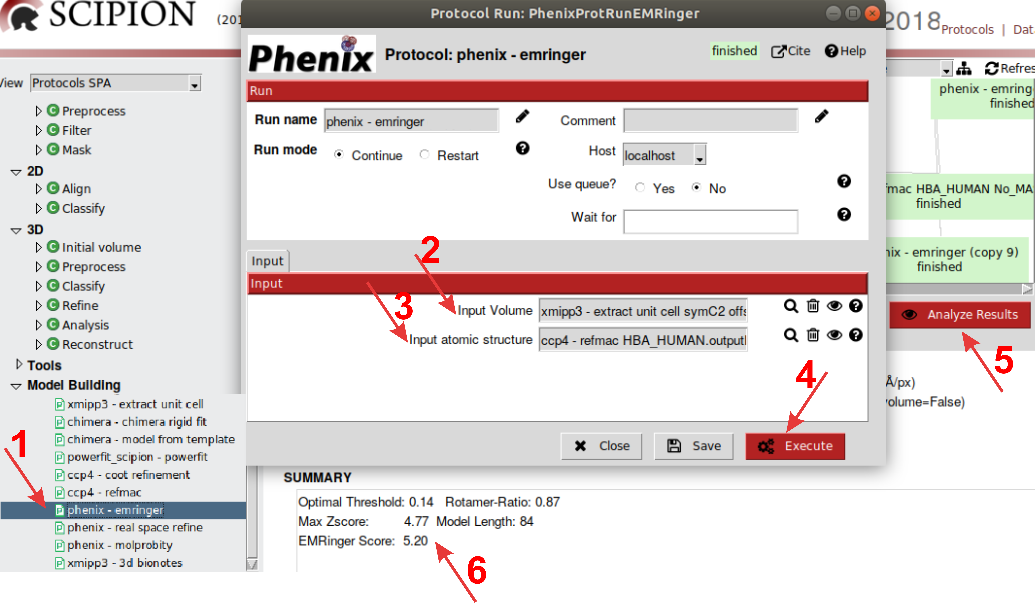
\includegraphics[width=0.85\textwidth]{Images/Fig34}
  \caption{Completing $EMRinger$ protocol form.}
  \label{fig:emringer_protocol}
  \end{figure}
 
 Run $EMRinger$ protocol and determine the respective score after running \iii{PowerFit item2}, $Chimera$ \ttt{rigid fit} ($model$ 2), $Coot$ refinement, $Phenix$ \ttt{real space refine} after $Coot$ (default conditions and last modification of form parameters), and $Refmac$ refinement with MASK before and after $Phenix$ \ttt{real space refine}. Considering $EMRinger$ \ttt{score}, does our \ttt{metHgb} $\alpha$ subunit $models$ seem to be OK? (Answers in appendix \ref{app:solutions}; \textbf{Question 8}). Try the same validation with $\beta$ subunit $models$. \\
 
 \item $MolProbity$:\\
 
 The atomic structure validation web service $MolProbity$, with better reference data has been implemented in the open-source CCTBX portion of $Phenix$ \citep{williams2018}. This widely used tool assesses $model$ geometry and quality at both global and local levels. Originally designed to evaluate structures coming from X-Ray diffraction and NMR, it does not take into account the quality of the fitting with a 3D density map.  The implementation in $Phenix$, nevertheless, includes the possibility of adding a volume and assessing the correlation in the real space.\\
 
 The assessment process that we have carried out with $EMRinger$ can also be done with $MolProbity$ in \scipion. We are going to validate the geometry of \ttt{metHgb} $\alpha$ subunit $models$ that we have generated along the modeling workflow. In each case, open the \scommand{phenix - molprobity} protocol (\ffigure{fig:molprobity_protocol} (1)), load the extracted unit cell volume (initial or generated by $Coot$) (2) wit its resolution (3) if you want to have real space correlation between map and $model$, load the $model$ atomic structure (4) and execute the protocol (5). In \ttt{Analyze results} (6) the same menu bars available in results section of $Phenix$ \ttt{real space refine} protocol are shown here. $MolProbity$ results bar include validation statistics. Protocol \ttt{SUMMARY} emphasizes the most relevant ones.\\
 
 \begin{figure}[H]
  \centering 
  \captionsetup{width=.7\linewidth} 
  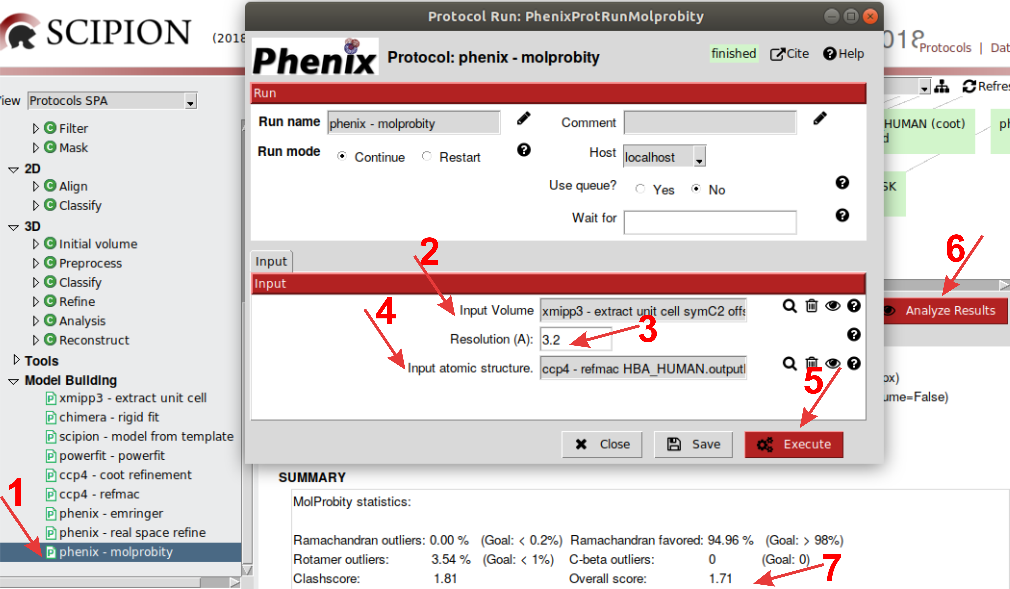
\includegraphics[width=0.85\textwidth]{Images/Fig35}
  \caption{Completing $MolProbity$ protocol form.}
  \label{fig:molprobity_protocol}
  \end{figure}
  
  Run $MolProbity$ protocol to obtain its statistics values after running \iii{PowerFit item2}, $Chimera$ \ttt{rigid fit} ($model$ 2), $Coot$ refinement, $Phenix$ \ttt{real space refine} (default conditions and last modification of form parameters) after $Coot$, and $Refmac$ refinement with MASK before and after $Phenix$ \ttt{real space refine}. In order to compare validation results of $models$ obtained along the modeling workflow, fill in the next table (\ttable{table:empty}) including, in addition to $MolProbity$ statistics, $EMRinger$ scores and \ccmask values obtained before. (Answers in appendix \ref{app:solutions}; \textbf{Question 9}). The same table (\ttable{table:empty}) can be completed for \ttt{metHgb} $\beta$ subunit (Appendix \ref{app:solutions}; \textbf{Question 10})\\
  
  \begin{sidewaystable}
   \caption{Validation statistics of human \ttt{metHgb} $\alpha$ subunit $model$. \ttt{RSRAC} stands for \ttt{Real Space Refine} after $Coot$. \ttt{Rama} stands for \ttt{Ramachandran}.}
   \centering\footnotesize
   \begin{tabular}{l c c c c c c c c}
   \hline\hline
   Statistic &  \thead{$Powerfit$\\ $item$ \#2} & \thead{$Chimera$\\ $model$ \#2} & $Coot$ & \thead{$Phenix$\\ \ttt{RSRAC}\\(default)} & \thead{$Phenix$\\ \ttt{RSRAC}\\(modified)} & \thead{$Refmac$\\ after $Coot$} & \thead{$Refmac$\\ after \ttt{RSRAC}\\(modified)} & \ttt{5NI1}\\ [0.5ex]
   \hline
   \ccmask \\
   $EMRinger$ \ttt{score} \\
   \ttt{RMS} (Bonds) \\
   \ttt{RMS} (Angles) \\
   \ttt{Rama favored} (\%) \\
   \ttt{Rama allowed} (\%) \\
   \ttt{Rama outliers} (\%) \\
   \ttt{Rotamer outliers} (\%) \\
   \ttt{Clashscore} \\
   \ttt{Overall score} \\
   \ttt{C$\beta$ deviations} \\
   \ttt{RMSD} \\[1ex] 
   \hline
   \end{tabular}
   \label{table:empty}
   \end{sidewaystable}
 
 
 Results compiled in this table indicate that statistics are uncorrelated. From the point of view of correlation in real space, the best $model$ was obtained from $Phenix$ \ttt{real space refine} (last modification of form parameters) after $Coot$. Considering $EMRinger$ \ttt{score}, the best $model$ derives from the whole workflow $Coot$ \ttt{->} $Phenix$ \ttt{real space refine} (default conditions). With $MolProbity$ \ttt{Overall score} as validation rule, the last step in the workflow could be suppressed because the best value was obtained after $Coot$ \ttt{->} $Phenix$ \ttt{real space refine} (last modification of parameters). We'd like to select the best $model$ and continue refining it in order to improve it as much as possible. Assuming that no one $model$ is perfect, how can we select the best one?\\ 


 \item $Model$ Comparison:\\
 
 The question posed in the previous item does not have an easy answer in the real world, in which we do not know the final atomic structure. In this tutorial, nevertheless, we know it and we can wonder how far we are of the atomic structure already published for this cryo-EM map. The question can be answered by comparing a) validation statistics that we have obtained for our $models$ with the statistics computed for the available $\alpha$ subunit in \ttt{PDB} structure \ttt{5NI1}, and b) the atomic structures themselves by overlapping.\\ 
    
  \begin{itemize}
  \item Comparison of validation statistics: \\
  
  Validation statistics of \ttt{metHgb} $\alpha$ subunit of \ttt{PDB} structure \ttt{5NI1} should be obtained as first step to compare them with our $models$ validation statistics. With this aim we are going to follow the next workflow:\\
  \begin{itemize}
    \item Protocol \scommand{import atomic structure}:\\
    Download from \ttt{PDB} structure \ttt{5NI1}\\
    
    \item Protocol \scommand{chimera operate} (Appendix \ref{app:chimeraOperate}):\\
    Similar to $Chimera$ \ttt{rigid fit}, $Chimera$ \ttt{operate} protocol allows to perform operations with atomic structures. We are going to use this protocol to save independently in \scipion the \ttt{metHgb} $\alpha$ subunit. Open the protocol  (\ffigure{fig:chimera_operate_protocol} (1)), complete the parameter \ttt{PDBx/mmCIF} including the atomic structure \ttt{5NI1} previously imported (2), and execute the protocol (3).      
    
    \begin{figure}[H]
    \centering 
    \captionsetup{width=.7\linewidth} 
    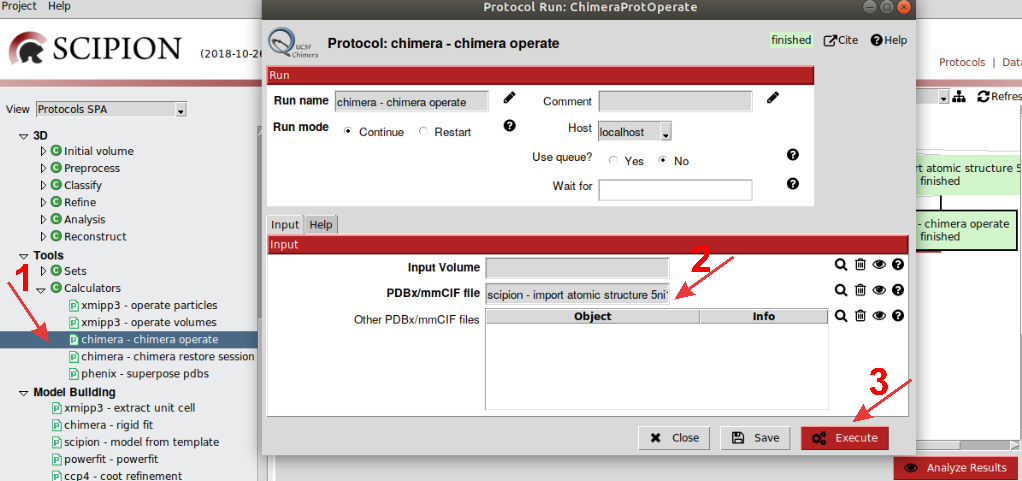
\includegraphics[width=0.90\textwidth]{Images/Fig36}
    \caption{Filling in $Chimera$ \ttt{operate} protocol form.}
    \label{fig:chimera_operate_protocol}
    \end{figure}
    
    The $Chimera$ graphics window will be opened with the structure \ttt{5NI1} as model number \#1. To save independently the structure of human \ttt{metHgb} $\alpha$ subunit (chain A), write in $Chimera$ command line:\\
    \ttt{split \#1}\\
    \ttt{scipionwrite model \#1.1}\\
    
    \item Protocol \scommand{powerfit}:\\
    Open $PowerFit$ protocol and follow the instructions above indicated. The structure saved in $Chimera$ operate will replace this time our previous $model$ (\ffigure{fig:powerfit_protocol} (2)). Select \ttt{item 2} as best fit.\\
    
    \item Protocol \scommand{chimera rigid fit}:\\
    Open again $Chimera$ \ttt{rigid fit} protocol and, following already indicated instructions, include this time \ttt{item 2}, the last fitted structure obtained with $PowerFit$ (\ffigure{fig:chimera_rigid_fit} (3)). After finishing the rigid fit of the extracted unit cell and \ttt{metHgb} $\alpha$ subunit from 5NI1 structure, you can save this fitted structure writing in $Chimera$ command line:\\
    \ttt{scipionwrite model \#2 refmodel \#1 saverefmodel 0}\\
    
    \item Validation protocols \scommand{phenix - emringer} and \scommand{phenix - molprobity}:\\
    Compute validation statistics with these two protocols for \ttt{metHgb} $\alpha$ subunit from \ttt{PDB} structure \ttt{5NI1}, write respective values in the previous table (\ttable{table:empty}), and compare them with the statistics of our $models$.
    
    Considering results shown in appendix \ref{app:solutions} (\textbf{Question 9}) for \ttt{metHgb} $\alpha$ subunit, we can conclude that published structures are not perfect and we are not very far from this published one. In fact, we have overcome every statistic except \ccmask. Then, the three different $models$ generated after $Coot$ refinement could be acceptable. \\

  \end{itemize}
 
  \item Comparison of atomic structures: \\
  
  $Phenix$ protocol \scommand{phenix - superpose pdbs} allows to compare two atomic structures by overlapping them. Root mean square deviation (RMSD) between the fixed structure (the published one) and one of our $models$ supports the classification of $models$ according to its proximity to the published model. Open $Phenix$ \ttt{superpose pdbs} protocol form (\ffigure{fig:superpose_pdbs_protocol} (1)), include the published structure of the \ttt{metHgb} $\alpha$ subunit as fixed structure (2), each one of the $models$ generated along the worflow (3) and execute the protocol (4). Finally, complete the \ttable{table:empty} with the value of RMSD obtained for each $model$. (Answers in appendix \ref{app:solutions}; \textbf{Question 9}).
  
  \begin{figure}[H]
    \centering 
    \captionsetup{width=.7\linewidth} 
    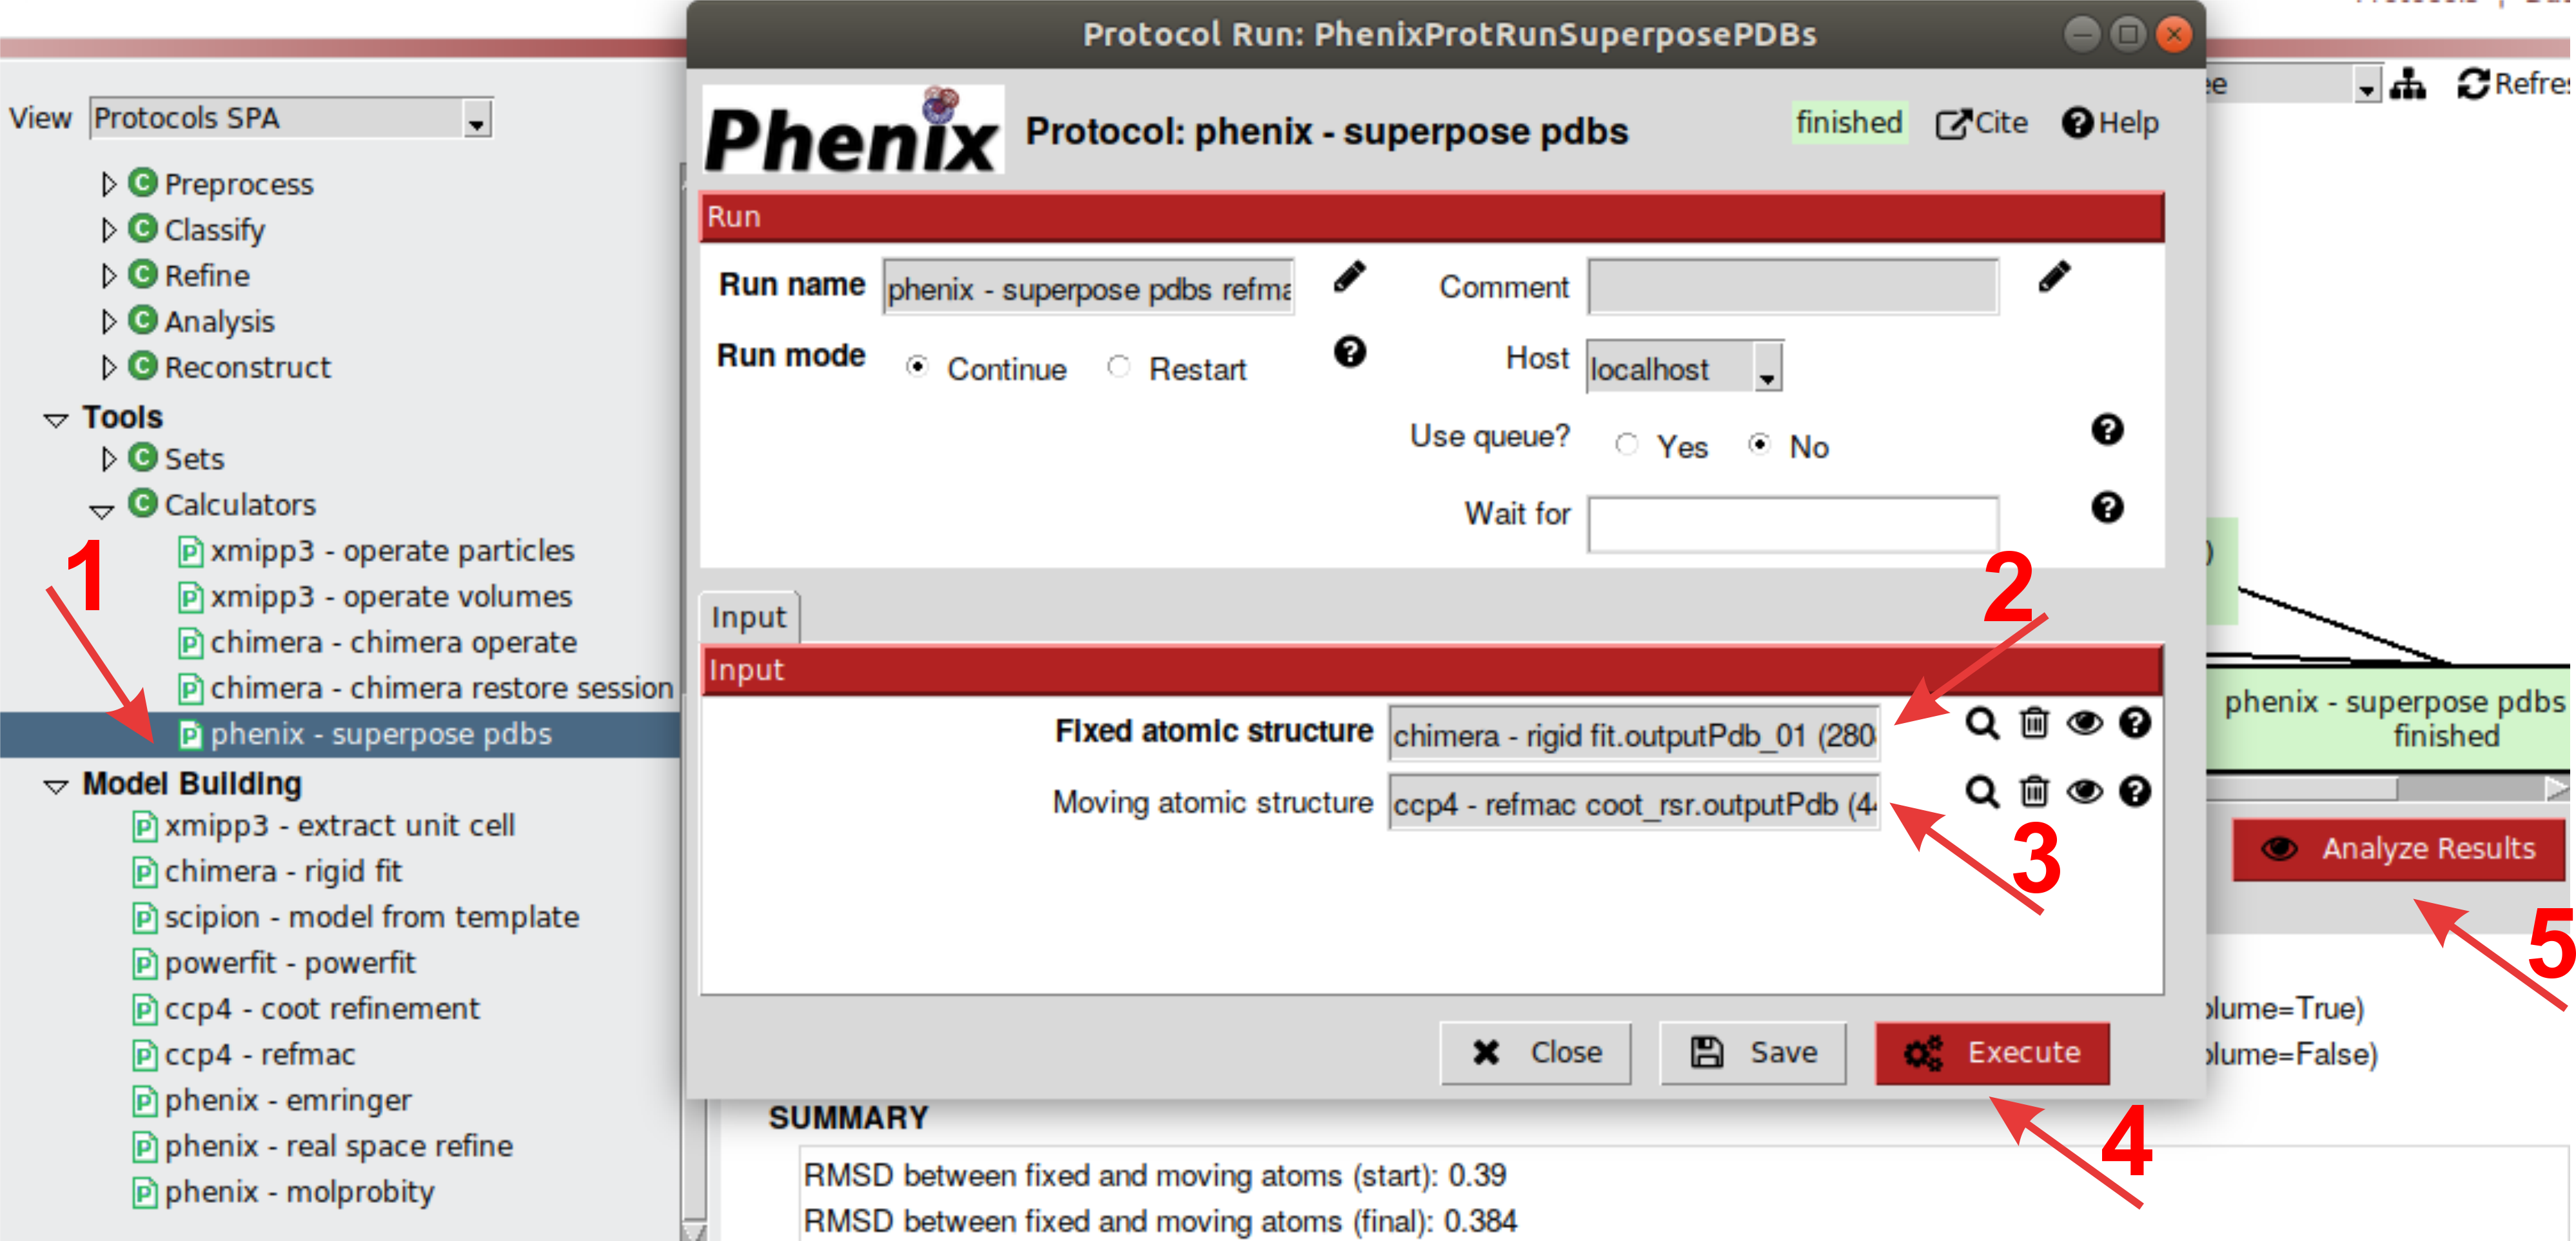
\includegraphics[width=0.90\textwidth]{Images/Fig37}
    \caption{Completing $Phenix$ \ttt{superpose pdbs} protocol form.}
    \label{fig:superpose_pdbs_protocol}
    \end{figure}
    
  You can check in $Chimera$ the fitted $model$ to the published structure by pressing \ttt{Analyze results} (\ffigure{fig:superpose_pdbs_protocol} (5)). Arrows of \ffigure{fig:superpose_pdbs_chimera} remark differing parts between both atomic structures. By opening these structures in $Coot$ you can see the difference between them.
 
   \begin{figure}[H]
    \centering 
    \captionsetup{width=.7\linewidth} 
    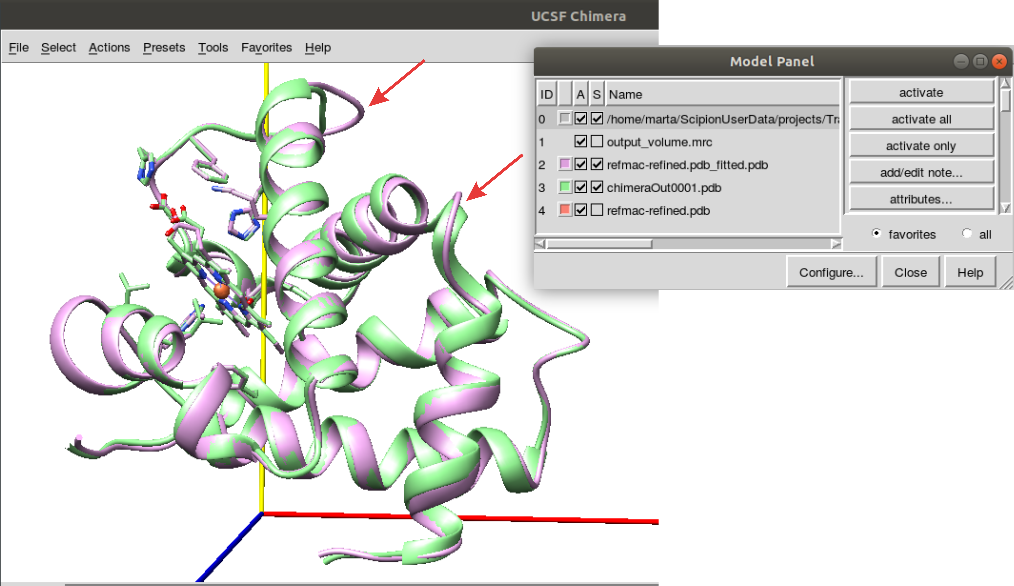
\includegraphics[width=0.90\textwidth]{Images/Fig38}
    \caption{$Model$ generated for \ttt{metHgb} $\alpha$ subunit superposed to published $\alpha$ chain of \ttt{5NI1} structure.}
    \label{fig:superpose_pdbs_chimera}
   \end{figure}
  
  
  \end{itemize}
 \end{itemize}
 
 A $model$ for \ttt{metHgb} $\alpha$ subunit has to be selected at the end of validation process. According to the statistics of \ttable{table:refmac_question_9} (Appendix \ref{app:solutions}; \textbf{Question 9}), $model$ obtained in the last step of modeling workflow ($Refmac$ after RSRAC (modified)) has been selected due to the smallest RMSD value, high value of $EMRinger$ \ttt{score}, quite high value of \ccmask and acceptable $MolProbity$ statistics. Follow a similar process to validate and select the $model$ generated for \ttt{metHgb} $\beta$ subunit. Appendix \ref{app:solutions} \textbf{Question 10} contains a statistics table for \ttt{metHgb} $\beta$ subunit, similar to that obtained for \ttt{metHgb} $\alpha$ subunit.\\
 
 In the real world, selected $models$ usually are the starting point to improve specific validation parameters by additional refinement. Since the improvement of certain parameters normally implies worsening of others, a final compromise solution has to be taken.\\

